% Kripke: payment\_gateway\_v1 (sinh tự động bởi core.reporter)
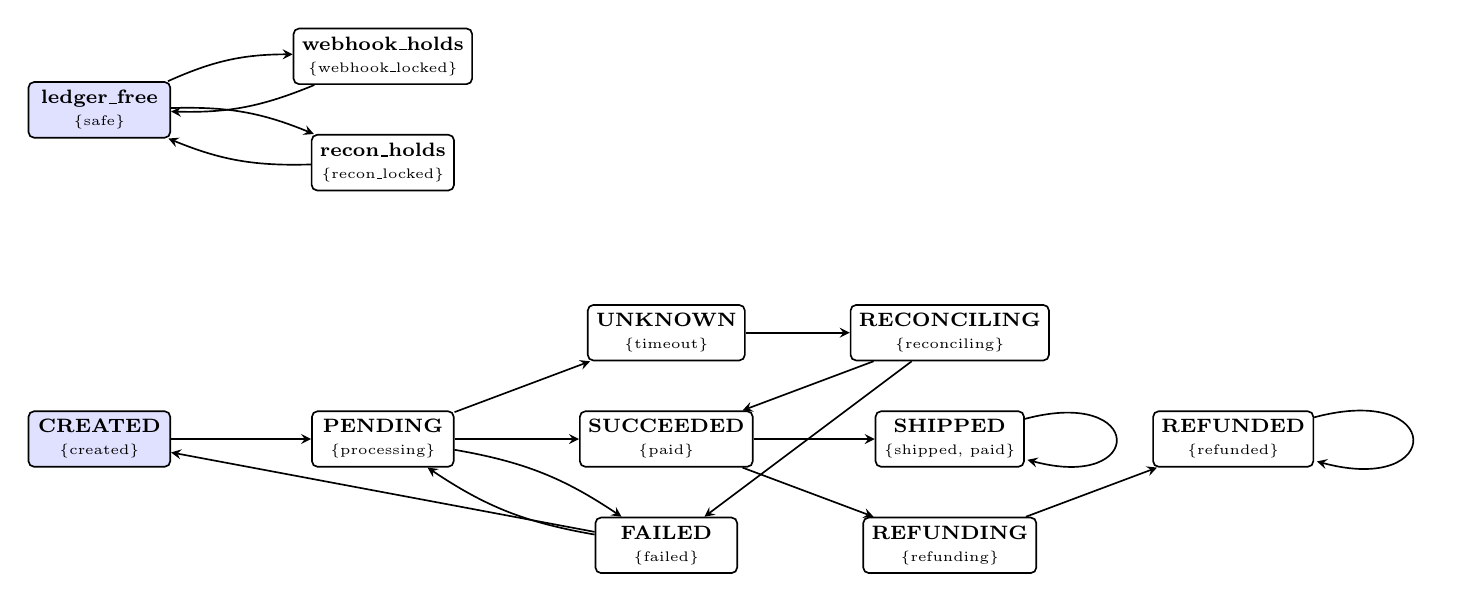
\begin{tikzpicture}[->,>=stealth,semithick,every node/.style={draw,rounded corners=2pt,align=center,font=\scriptsize,inner sep=3pt,minimum width=18mm}]
  \node[fill=blue!12] (n_ledger_free) at (0.00,-0.68) {\textbf{ledger\_free}\\{\tiny \{safe\}}};
  \node[fill=white] (n_webhook_holds) at (3.60,-0.00) {\textbf{webhook\_holds}\\{\tiny \{webhook\_locked\}}};
  \node[fill=white] (n_recon_holds) at (3.60,-1.35) {\textbf{recon\_holds}\\{\tiny \{recon\_locked\}}};
  \node[fill=blue!12] (n_CREATED) at (0.00,-4.86) {\textbf{CREATED}\\{\tiny \{created\}}};
  \node[fill=white] (n_PENDING) at (3.60,-4.86) {\textbf{PENDING}\\{\tiny \{processing\}}};
  \node[fill=white] (n_UNKNOWN) at (7.20,-3.51) {\textbf{UNKNOWN}\\{\tiny \{timeout\}}};
  \node[fill=white] (n_RECONCILING) at (10.80,-3.51) {\textbf{RECONCILING}\\{\tiny \{reconciling\}}};
  \node[fill=white] (n_SUCCEEDED) at (7.20,-4.86) {\textbf{SUCCEEDED}\\{\tiny \{paid\}}};
  \node[fill=white] (n_FAILED) at (7.20,-6.21) {\textbf{FAILED}\\{\tiny \{failed\}}};
  \node[fill=white] (n_SHIPPED) at (10.80,-4.86) {\textbf{SHIPPED}\\{\tiny \{shipped, paid\}}};
  \node[fill=white] (n_REFUNDING) at (10.80,-6.21) {\textbf{REFUNDING}\\{\tiny \{refunding\}}};
  \node[fill=white] (n_REFUNDED) at (14.40,-4.86) {\textbf{REFUNDED}\\{\tiny \{refunded\}}};
  \draw[bend left=12] (n_ledger_free) to (n_webhook_holds);
  \draw[bend left=12] (n_ledger_free) to (n_recon_holds);
  \draw[bend left=12] (n_webhook_holds) to (n_ledger_free);
  \draw[bend left=12] (n_recon_holds) to (n_ledger_free);
  \draw[] (n_CREATED) to (n_PENDING);
  \draw[] (n_PENDING) to (n_SUCCEEDED);
  \draw[bend left=12] (n_PENDING) to (n_FAILED);
  \draw[] (n_PENDING) to (n_UNKNOWN);
  \draw[] (n_UNKNOWN) to (n_RECONCILING);
  \draw[] (n_RECONCILING) to (n_SUCCEEDED);
  \draw[] (n_RECONCILING) to (n_FAILED);
  \draw[] (n_SUCCEEDED) to (n_SHIPPED);
  \draw[] (n_SUCCEEDED) to (n_REFUNDING);
  \draw[bend left=12] (n_FAILED) to (n_PENDING);
  \draw[] (n_FAILED) to (n_CREATED);
  \draw[] (n_SHIPPED) edge[loop right] (n_SHIPPED);
  \draw[] (n_REFUNDING) to (n_REFUNDED);
  \draw[] (n_REFUNDED) edge[loop right] (n_REFUNDED);
\end{tikzpicture}
